% !TEX root = ../main.tex
% !TeX spellcheck = fr_FR

\chapter{Optimisation des ressources d'un \ac{LLN} avec un cache intelligent}
\label{cache}

\epigraph{There are only two hard problems in Computer Science: cache invalidation and naming things.}{Phil Karlton}

\minitoc

Ce chapitre présente comment optimiser l'utilisation des ressources d'un \ac{LLN} par l'emploi d'un service de mise en cache qui adapte son comportement en fonction des conditions du \ac{LLN}.

La section~\ref{cache:introduction} introduit les mécanismes applicatifs mis en place au niveau de la passerelle et les contraintes liées à leur gestion.

La section~\ref{cache:related} présente l'état de l'art sur les différentes solutions de mises en cache visant à optimiser l'utilisation des ressources d'un réseau.

La section~\ref{cache:rpca} présente la contribution de ce chapitre en détaillant son architecture, ses modèles théoriques et les méthodes d'optimisation multi-objectifs employées.

La section~\ref{cache:validation} couvre la validation expérimentale du système proposé en présentant les gains obtenus.

La section~\ref{cache:conclusion} conclut ce chapitre et présente les ouvertures possibles de ces travaux.

\section{Introduction}
\label{cache:introduction}

Les \ac{LLN}s ont pour objectif de fournir des relevés et des mesures sur leur environnement à des services à valeur ajoutée.
Comme vu dans la section~\ref{gw:app_layer}, la passerelle a pour rôle d'assurer l'interface entre un \ac{LLN} et ces services tiers.

\subsection{Objectifs d'un \acl{RPC}}

Pour remplir son rôle d'interface applicative, la passerelle utilise un \acf{RPC} qui est un logiciel s'exécutant au niveau de la passerelle et qui intercepte l'ensemble des requêtes applicatives qu'elle reçoit.
Un \ac{RPC} a plusieurs objectifs: traduire les requêtes entre différents protocoles; gérer les requêtes admises dans le \ac{LLN}; accélérer leur traitement tout en réduisant la consommation des ressources.

\subsubsection*{Traduction inter protocoles}

Les nœuds capteurs mettent en jeu des protocoles applicatifs hétérogènes et supporter tous ces protocoles au niveau de chaque client serait coûteux et difficile à maintenir.
Ainsi la passerelle utilise un mécanisme de \emph{traduction} pour traduire les requêtes venant d'un protocole classique (par exemple \ac{HTTP}) vers un protocole supporté par les nœuds du \ac{LLN}s (par exemple \acl{CoAP}).

\subsubsection*{Reverse-proxy}

Les nœuds d'un \ac{LLN} peuvent recevoir un flot trop important de requêtes applicatives qui aura un impact fort sur la consommation de leurs ressources.
Afin de limiter ce type de situation, un reverse-proxy peut être utilisé afin de répondre à ces requêtes à la place des nœuds.

Un reverse-proxy est un logiciel qui se place entre un ou plusieurs serveurs et qui répond aux requêtes destinées à ces serveurs, à leur place en faisant les traitements nécessaires.
Ce fonctionnement est transparent pour les clients qui communiquent avec le reverse-proxy comme s'ils communiquaient avec les serveurs originaux.

Ce type d'architecture est utilisé par une grande partie des sites web les plus consultés du monde afin de router dynamiquement les requêtes vers différents serveurs afin de répartir la charge~\cite{reese2008nginx,guinard2010resource}.

\subsubsection*{Cache}

Si un reverse-proxy n'a pas de cache, alors il se contente de faire suivre la requête vers le serveur visé.
Dans le cas d'un \ac{LLN}, le traitement d'une requête est long, car les latences entre les nœuds sont élevées (mécanisme de cycle de veille, réémissions sur le canal, etc.).
D'autre part, lorsqu'une même requête est effectuée plusieurs fois sans que la réponse ne change, un \ac{LLN} consomme de la bande passante et de l'énergie inutilement.

Ainsi, la passerelle utilise un mécanisme de cache afin d'économiser les ressources d'un \ac{LLN} et accélérer le traitement des requêtes.

\subsection{Fonctionnement d'un \ac{RPC}}

Le but d'un \ac{RPC} est de réutiliser une réponse obtenue précédemment afin de répondre à une requête en cours en évitant de solliciter le \ac{LLN}.
Pour fonctionner, un \ac{RPC} garde en mémoire une table de correspondance entre une \ac{URI} et une réponse.
Quand une nouvelle requête arrive, cette table est utilisée afin de la servir comme réponse sans solliciter de nouveau le serveur dont elle est issue.

Il existe deux mécanismes principaux: un mécanisme par fraîcheur (``Freshness model'' en anglais) et un mécanisme par validation.

\paragraph{Fraîcheur des réponses}

Une réponse à une requête qui est suffisamment ``fraîche'' peut être utilisée par le \ac{RPC} pour répondre à de nouvelles requêtes.
Un nœud capteur peut définir le temps maximal pendant lequel un \ac{RPC} peut réutiliser une réponse en utilisant une option (Max-Age).
Tant que la réponse n'est pas restée dans le \ac{RPC} plus longtemps que cette durée, elle est considérée comme ``fraîche'' et le \ac{RPC} l'utilise afin d'économiser les ressources du serveur d'origine.
De plus, un nœud serveur qui ne veut pas que cette réponse soit mise en cache peut utiliser cette option en lui donnant une valeur nulle.
Ce mécanisme est par exemple utile pour mettre en cache des mesures qui ne changent pas significativement au cours du temps (température, pluviométrie, etc.)~\cite{cachingbestpractices}.

\paragraph{Revalidation des réponses}

Il peut arriver qu'une réponse soit toujours valide, mais ne soit plus considérée comme fraîche car son temps de validité a expiré.
Dans ce cas, la réponse peut être revalidée par l'utilisation d'un mécanisme d'\ac{ETag}.

Un \ac{ETag} est un identifiant unique assigné par le serveur applicatif à chaque version d'une ressource accessible par une \ac{URI}. 
Si la ressource en question est modifiée, un nouveau \ac{ETag} différent du précédent lui est assigné. 
Ainsi, un \ac{RPC} peut comparer deux \ac{ETag} successifs et vérifier s'ils correspondent à deux versions identiques d'une même ressource, et ainsi savoir si une demande peut être honorée par une réponse en cache ou pas.

Lorsqu'un client effectue une nouvelle requête, il peut indiquer quel était l'\ac{ETag} de la précédente réponse obtenue.
Dans le cas où elle est toujours valide, le \ac{RPC} peut la revalider sans solliciter les nœuds.
Dans le cas où le \ac{RPC} a besoin de la revalider avec le serveur d'origine, il envoie l'\ac{ETag} dans la requête.
Si la réponse est toujours valide, un simple code de retour est renvoyé ce qui permet à un nœud de revalider la réponse sans la transférer entièrement.
Dans le cas contraire, la nouvelle réponse avec un nouveau \ac{ETag} est transférée normalement.

Ce mécanisme est par exemple utile pour mettre en cache des notifications ou des alertes sur un état.
Un état n'a pas de durée de vie connue à l'avance, car il peut changer n'importe quand, mais la réponse qu'il envoie sera revalidée en l'absence de changements.

\subsection{Problématique des reverse proxy}

L'utilisation d'un \ac{RPC} requiert de le configurer correctement en raison de son rôle clé dans la gestion des requêtes applicatives.
Un \ac{RPC} est le logiciel en charge de la traduction des requêtes applicatives, ainsi s'il tombe en panne, cette traduction n'est plus assurée et les services tiers ne peuvent plus accéder aux \ac{LLN}s par des requêtes usuelles.
De plus, si un attaquant parvient à prendre le contrôle d'un \ac{RPC} il peut effectuer des attaques \ac{MITM} qui peuvent à la fois compromettre les données, mais également permettre une attaque au déni de sommeil contre les nœuds afin d'épuiser leurs ressources.

D'autre part, un serveur applicatif contraint n'est pas toujours obligé de spécifier un temps de vie pour chaque ressource qu'il offre.
Or si la quantité de requêtes pour ce nœud devient importante, l'absence de mécanisme de mise en cache dégradera les performances et consommera beaucoup de ressources.
Ainsi quand un serveur applicatif ne le rejette pas explicitement, un \ac{RPC} peut être légitimement mandaté pour spécifier des temps de vie dans le but d'alléger la charge sur un nœud applicatif.
Cependant, le choix de la durée de vie pour une requête n'est pas trivial: un temps de vie trop court rendra la mémoire cache inefficace, car invalidée rapidement tandis qu'un temps de vie trop long risquera de donner des valeurs obsolètes.
Dans un cas extrême, un reverse-proxy peut peupler son cache de manière permanente sans invalider aucune réponse et ainsi aucune requête applicative ne pourrait passer ce qui donnerait à la fois de grandes économies d'énergie et des réponses obsolètes rapidement.
Ainsi un mécanisme visant à trouver des temps de validité optimaux pour chaque requête doit tenir compte de ces deux objectifs concurrents.
Le reste de ce chapitre se concentrera sur les moyens d'obtenir ces temps de validité optimaux.

\section{État de l'art}
\label{cache:related}

Les \ac{RPC} peuvent être modélisés par des caches dits \acl{TTL} où les réponses restent valides pendant un temps donné puis sont retirées du cache~\cite{berger2014exact}.
Ce cadre théorique mesure les performances attendues, mais ne donne cependant pas de critères sur comment choisir ces temps de vie en fonction d'un contexte donné.

\subsection{\ac{RPC} pour les \ac{LLN}s}

Les \ac{RPC} sont utilisés dans les \ac{LLN}s avec des architectures similaires à celles des sites web classiques~\cite{colitti2011integrating, colitti2011rest}.
Cependant, le calcul des temps de vie n'est pas spécifié dans les implémentations et dépend des choix des utilisateurs.

L'utilisation de cache au niveau des routeurs intermédiaires du \ac{LLN} est également une technique explorée~\cite{duquennoy2011leveraging}, cependant les paramètres de gestion des temps de validité ne prennent généralement pas en compte les métriques d'un nœud (réserve de batterie) ou même du \ac{LLN} entier (temps de vie).

\subsection{Optimisation des ressources basée sur les temps de vie}

Des méthodes heuristiques sont employées dans les \ac{RPC} \ac{HTTP} afin de configurer des temps de vie pour les réponses aux requêtes qui ne spécifient pas un temps de vie par elle-même~\cite{michel1998adaptive}.
Ces heuristiques sont très hétérogènes, mais se basent le plus souvent sur les dates de modification d'une \ac{URI} pour fournir un temps de vie d'une réponse~\cite{gourley2002http}.
En outre, elles ne sont utilisées que lorsque le temps de vie n'est pas explicité par le serveur d'origine lui-même et ne peut pas dépasser une certaine durée sans l'envoi d'un avertissement à l'utilisateur final~\footnote{Fixée à 24 heures dans le cas de \ac{HTTP}~\cite{rfc7234}.}.

Ces approches ne sont pas satisfaisantes pour les \ac{LLN}s, car le calcul des temps de vie ne se fait que sur l'\ac{URI} et néglige le contexte propre à chaque nœud et en particulier, la quantité de paquets qu'il peut gérer et ses réserves d'énergies.

\subsection{Optimisation des ressources énergétiques par cache}

Les caches sont utilisés dans les \ac{CCN} pour distribuer le contenu dans le réseau aux meilleurs emplacements afin de répondre aux requêtes des utilisateurs efficacement.
Les économies d'énergies sont des problématiques présentes au sein de cette communauté et des études ont montré comment utiliser les caches de manière optimale afin d'économiser de l'énergie.

Llorca~\cite{llorca2013dynamic} utilise des mécanismes distribués pour placer des caches de manière optimale dans un réseau afin d'économiser de l'énergie, or l'approche recherchée dans ce chapitre se concentre sur une architecture centralisée autour du \ac{RPC}.
D'autres approches~\cite{li2013energy,choi2012network} utilisent un mécanisme de popularité d'un contenu afin de déterminer si une ressource doit être conservée ou non.
Cependant, ces approches ne se concentrent que sur la présence d'un contenu dans un cache et ne spécifient pas explicitement un temps de vie pour cette ressource qui est l'objectif recherché.

\section{Reverse Proxy Cache Adaptatif}
\label{cache:rpca}

Un \ac{RPCA} est un \ac{RPC} qui configure pour chaque réponse de requête, un temps de vie optimal.
Son objectif est de trouver en fonction des objectifs de durée de vie d'un \ac{LLN} quelle est la qualité de service maximale qui peut être obtenue.
Réciproquement, pour une qualité de service donnée, un \ac{RPCA} donne les meilleurs objectifs de durée de vie possible.

Afin de trouver les temps de vie acceptables pour chaque ressource, un \ac{RPCA} modélise la durée de vie d'un \ac{LLN} et la satisfaction des utilisateurs comme deux fonctions des temps de vie des réponses qui doivent être optimisées en même temps.
Puis le \ac{RPCA} résout le problème multi-objectifs afin de fournir les temps de vie acceptables.
La résolution d'un problème multi-objectifs étant coûteuse, il est important de trouver efficacement un ensemble de solutions afin de changer rapidement les temps de vie au cas où les hypothèses viendraient à changer.

\subsection{Architecture}
\label{cache:architecture}

\begin{figure}[ht]
  \centering
  \begin{tikzpicture}

  % définition des styles
  \tikzstyle{visible}=[draw, fill=blue!50]
  \tikzstyle{hidden}=[ draw, fill=gray!20]
  \tikzstyle{router}=[circle, draw, fill=orange!50,text=black]
  \tikzstyle{child}=[circle, draw, fill=yellow!50,text=black]
  \tikzstyle{root}=[circle, draw, fill=red!50,text=black]

  % les nœuds
  \node[draw] (gw) {Reverse Proxy Cache Adaptatif};

  \node[visible, below=of gw] (adapt) {Calcul des durées de validité optimales};


  % Réseau contraint
  \node[root] (1) at (-4, 0) {};
  \node[router] (2) at (-5, 1) {};
  \node[child] (3) at (-5, -1) {};
  \node[child] (4) at (-6, 2) {};
  \node[child] (5) at (-6, 0) {};

  % \node[cloud, cloud puffs = 10, minimum width = 4cm, draw, fill = gray!10] (cloud) at (5,0) {Réseau local};
  \node[draw] (cloud) at (5,0) {Réseau local};

 \node [fit=(1) (2) (3) (4) (5), rounded corners, draw=black!50] (lln) {};
 \node [below=.3 cm of lln] {LLN};

\path

  % Réseau contraint
  (gw) edge[<->, thick] node [above] {$r_u$} (1)
  (1) edge[<->] (2)
  (1) edge[<->] (3)
  (2) edge[<->] (4)
  (2) edge[<->] (5)

  % Réseau conventionnel
  (gw.east) edge[<->, ultra thick] node [above] {$T_u$} (cloud)

  % Cache
  (gw) edge[->,very thick, bend left=10] node [midway,right] {$(\mathcal{T}, \mathcal{L})$} (adapt)
  (adapt) edge[->,very thick, bend left=10] node [left] {$\mathcal{C}$} (gw)
  ;

  \end{tikzpicture}

  \caption{Architecture du \ac{RPCA}}

  \label{cache:fig:schema}
\end{figure}

Un \ac{RPCA} se place au niveau de la passerelle et intercepte comme le ferait un \ac{RPC} classique les requêtes applicatives visant le \ac{LLN}.
Afin d'éviter les problèmes liés à la synchronisation des caches, il est supposé qu'il n'y a qu'un seul \ac{RPCA} pour l'ensemble des nœuds.
Cette hypothèse est assez réaliste, car dans les déploiements usuels, la passerelle est le point d'entrée unique vers un \ac{LLN}.

Soit $u$, l'\ac{URI} de la requête courante et $c_u$ le temps de validité associé à la réponse de cette valeur.
Une requête visant une \ac{URI} $u$, venant de l'extérieur, en cache depuis moins de $c_u$ sera traitée par le \ac{RPC} sans solliciter le \ac{LLN}.
Soit $\mathcal{C}$ l'ensemble de tous les $c_u$ que la passerelle gère.

Pour fonctionner, un \ac{RPCA} a besoin d'estimer efficacement la durée de vie d'un \ac{LLN}, or comme le montre le chapitre~\ref{supervision}, la connaissance de la topologie est importante pour avoir des estimations correctes.
Soit $\mathcal{T}$, la topologie du \ac{LLN} et $\mathcal{L}$ la durée de vie souhaitée pour le \ac{LLN}.
Il est supposé dans le reste de ce chapitre que la topologie du réseau est connue du \ac{RPCA}.

\subsection{Calcul théorique de l'impact du cache sur l'intensité des requêtes}
\label{cache:simple}

Le nombre moyen de requêtes reçues à destination de l'\ac{URI} $u$ est modélisé par un processus de Poisson de paramètre $\lambda_u$: $T_u = \frac{1}{\lambda_u}$ est le temps moyen entre deux requêtes successives vers $u$.
Le \ac{RPCA} agit sur les requêtes entrantes afin que le temps moyen entre deux requêtes pour la ressource $u$ soit de $r_u$.

Si le \ac{RPCA} a une valeur stockée qui est encore valide, il répond directement à la demande d'un client.
Sinon, si la valeur requise n'est pas présente ou plus âgée que $c_u$, il transfère la demande au serveur du \ac{LLN} hébergeant cette \ac{URI} afin de le revalider ou à défaut d'avoir une nouvelle réponse.

Il est supposé que les temps caractéristiques de traitement d'une requête par le \ac{LLN} sont très petits devant les temps $c_u$ et $T_u$ afin de supposer que quand une requête traverse le cache (miss), toutes les requêtes qui arrivent dans l'intervalle $c_u$ qui suit seront servies par le cache (hit).

Soit $m_u$ la probabilité qu'une requête pour l'\ac{URI} $u$ ne puisse pas être satisfaite par le \ac{RPCA}.

À chaque requête qui traverse le cache (miss) est associée une fenêtre temporelle de taille $c_u$ pendant laquelle toutes les requêtes sont traitées par le cache.
Ces fenêtres ne se chevauchent pas~\footnote{L'article original~\cite{leone2013optimizing} fait une modélisation différente en supposant que le temps de vie est réinitialisé à chaque nouvelle requête.}: les requêtes traversantes sont forcément espacées d'au moins $c_u$.

Si les requêtes venues de l'extérieur arrivent avec une intensité $\lambda_u$, le nombre de requêtes observées pendant un intervalle $c_u$ est en moyenne $\lambda_u$ $c_u$.
Donc, à chaque requête qui traverse est associée (en moyenne) $\lambda_u$ $c_u$ requêtes cache.
La proportion de miss et de hit est donc:

\begin{align}
  m_u &= \frac{1}{1 + \lambda_u c_u}
  \label{cache:eq:cache_miss}\\
  h_u &= 1 - m_u = \frac{\lambda_u c_u}{1 + \lambda_u c_u}
  \label{cache:eq:cache_hit}
\end{align}
 
Ainsi le \ac{LLN} reçoit une intensité de $m_u \lambda_u$ requêtes.
Ce processus n'est pas un processus de Poisson, en particulier, deux requêtes sont toujours espacées d'au moins $c_u$.
Cependant, le calcul du temps moyen entre deux requêtes est toujours l'inverse de l'intensité.
Ainsi, $r_u$ se met sous la forme:

\begin{align}
  r_u &= \frac{1}{m_u \lambda_u} = T_u \left (1 + \frac{c_u}{T_u} \right) = T_u + C_u 
  \label{cache:eq:r_u}
\end{align}

Lorsque $c_u \rightarrow 0$, $r_u \rightarrow T_u$ ce qui correspond à un comportement où le cache est absent.
D'autre part, quand $c_u$ devient grand devant $T_u$, $r_u$ tend vers $c_u$.

%%% Contenu avant Fabien

% Ainsi, $m_u$ correspond à la probabilité que le temps entre chaque arrivée d'une requête soit plus grande que $c_u$:

% \begin{align}
%   m_u = \int_{c_u}^{\infty} \frac{e^{-\frac{t}{T_u}}}{T_u} {\textrm{d}}t = e^{-\frac{c_{u}}{T_u}}.

% \end{align}

% Le ``hit ratio'' $h_u$, c'est à dire la probabilité que la réponse pour l'\ac{URI} $u$ soit servie par le cache est le complémentaire de $m_u$:

% \begin{equation}
%   h_u = 1 - e^{-\frac{c_u}{T_u}}
%   
% \end{equation}

% Étant donné que la demande pour la ressource $u$ arrive en moyenne chaque $T_u$, la durée moyenne $r_u$ entre deux requêtes consécutives arrivant dans le \ac{LLN} est donc:

% % \begin{align}
% %     r_u = \left\{ \begin{array}{ll} \lceil{\frac{c_u}{T_u}}\rceil
% %     T_u & {\textrm{si}\:} T_u\leq c_u\\ T_u &  {\textrm{sinon}}.  \end{array} \right.
% %     
% % \end{align}

% % Si $c_u < T_u$, la réponse mise en cache deviendra non fraîche avant d'être ré-utilisée.
% % Si $c_u > T_u$, alors le cache sera efficace et le temps entre deux requêtes touchant le \ac{LLN} sera plus grand: $r_u > T_u$.

% \begin{align}
%   r_u = \frac{T_u}{m_u}
% \end{align}

\subsection{Modélisation de la durée de vie}

Un \ac{RPCA} a besoin d'avoir une estimation de la consommation énergétique afin d'établir une estimation de la durée de vie pour savoir si une configuration $\mathcal{C}$ est admissible.

Cette section détaille le modèle approché utilisé pour obtenir une estimation de la consommation énergétique.
Comme pour le chapitre précédent, cette modélisation se concentre sur la consommation de l'interface radio qui est la principale source de consommation énergétique d'un nœud capteur~\cite{molina2010energy} et néglige celle des autres composants (\ac{CPU}, flash, etc.).

Il est supposé que les nœuds du \ac{LLN} sont à la fois des serveurs applicatifs et des routeurs (en fonction de la topologie) et que leur batterie est une réserve fixe non renouvelable.

\subsubsection{Énergie résiduelle}

Pour un \ac{LLN} utilisant une source d'énergie non rechargeable initiale de $E_0$, l'énergie résiduelle $E_r$ à un instant $T$ est donnée par:

\begin{align}
  E_r(T) = E_0 - \int_0^T P(t) \mathrm{d}t
  \label{contikimac:eq:residual_energy}
\end{align}

où $E_0$ est l'énergie initiale du nœud considéré (en joules) et $P(t)$ est la puissance consommée (en watts) par le système au cours du temps.
La durée de vie théorique du \ac{LLN} est obtenue avec un modèle linéaire~\cite{chen2005lifetime} qui peut être calculé en utilisant les $r_u$ obtenus pour une configuration $\mathcal{C}$.

\subsubsection{États de transmission d'un nœud}

La radio d'un nœud peut être dans 4 états possibles: transmission, réception, en veille ou en écoute du canal.
Ainsi, la consommation énergétique globale d'un nœud est obtenue en sommant les parts liées aux différents états:

\begin{align}
  % \Omega &= \Omega_\sleep + \Omega_\listen + \Omega_\tx + \Omega_\rx\\
  \int_0^T P(t) \mathrm{d}t &= \int_0^T P_\sleep \alpha_\sleep(t) \mathrm{d}t + \int_0^T P_\listen \alpha_\listen(t) \mathrm{d}t + \int_0^T P_\tx \alpha_\tx(t) \mathrm{d}t + \int_0^T P_\rx \alpha_\rx(t) \mathrm{d}t\\
  &= \alpha_\sleep P_\sleep + \alpha_\listen P_\listen + \alpha_\tx P_\tx + \alpha_\rx P_\rx
  \label{contikimac:eq:omega_tot}
\end{align}

où: $\alpha_\sleep$ est la proportion de temps passé en sommeil; $\alpha_\listen$ est la proportion de temps passé en écoute du canal; $\alpha_\rx$ est la proportion liée à la réception et $\alpha_\tx$ est la part liée à la transmission.

Dit autrement, $\Omega_X = \alpha_X P_X$ est la part de puissance liée à un état donné $X$ où $P_X$ est la puissance consommée dans l'état $X$ qui est supposée constante au cours de la vie d'un nœud et $\alpha_X$ la proportion de temps passé en état $X$.
La puissance consommée dans un état donné $X$ étant constante, $P_X$ peut être sortie de l'intégrale.
De plus, puisque $\alpha_X(t)$ est une fonction créneau, son intégrale peut être simplifiée et donne simplement la proportion de temps passé dans l'état $X$.

Les sections suivantes se concentrent sur les moyens de modéliser et d'estimer les différents $\alpha_X$

\subsection{Modélisation des temps moyens de transmission et de réception avec ContikiMAC}

ContikiMAC est un mécanisme de cycle de veille disponible dans Contiki-OS~\cite{dunkels11contikimac} qui est notamment utilisé dans les nœuds capteurs pour économiser de l'énergie (cf. \ref{supervision:contikimac}).
Ce mécanisme de cycle de veille construit au-dessus de \ieee{} permet au nœud d'éteindre et  d'allumer sa radio périodiquement~\footnote{Par défaut toutes les 125 ms} pour consulter l'activité du canal.

Les réveils de nœuds voisins peuvent être désynchronisés, ainsi la source d'une trame devra l'envoyer à plusieurs reprises ({\em strobing}) jusqu'à la réception d'un acquittement ou bien le nombre maximal de retransmissions possibles.
Lors d'un réveil, si un nœud détecte que le canal est occupé, il reste éveillé jusqu'à la réception de la trame entière.
Si ce nœud est le destinataire de cette trame, il reste éveillé pour le recevoir entièrement sinon il éteint sa radio.
Des mécanismes complémentaires de ``phase-locking'' sont mis en place afin de réduire les envois répétés de paquets par l'expéditeur cependant ces optimisations n'offrent pas de garanties.
Il est supposé ici que les paquets ne sont pas perdus en raison de collisions ou de congestions, car le trafic est jugé suffisamment faible.

$T_\cycle$ est défini comme la durée entre deux phases actives consécutives et $T_\sleep$ comme la durée de la phase de sommeil du nœud considéré.
La durée de la phase active d'un nœud en l'absence de transmission peut être évaluée comme: $T_\act = T_\cycle - T_\sleep$.

\subsubsection{Transmission d'un paquet}
\label{contikimac:transmission}

Les serveurs et routeurs transmettent des trames liées aux requêtes et aux réponses à travers le \ac{LLN}.
La durée de transmission d'un paquet de requête est définie comme: $T_\req = \frac{L_\req}{R}$ et celui de la réponse: $T_\ans = \frac{L_\ans}{R}$,  où $L_\req$ et $L_\ans $ sont les tailles de paquet de la requête et de la réponse respectivement et $R$ est le débit de transmission des nœuds.

D'après le protocole ContikiMAC~\cite{dunkels11contikimac} quand un nœud transmet un paquet $\pkt$ (une requête $\req$ ou une réponse $\ans$), il reste durant $T_{\pkt, \txtx}$ en transmission et pour une période $T_{\pkt, \txrx}$ en réception afin de recevoir le paquet \ac{ACK} du destinataire.
Ces périodes de temps peuvent changer en fonction de la synchronisation des réveils:

\paragraph{Cas favorable}

\begin{align}
  T_{\pkt, \txtx} &= T_\pkt
  \label{contikimac:eq:pck_txtx_best} \\
  T_{\pkt, \txrx} &= T_\ack
  \label{contikimac:eq:pck_txrx_best}
\end{align}

où $T_\pkt$ indique un paquet générique qu'il soit une requête  $T_\req$ ou une réponse $T_\ans$.
$T_\ack$ est le temps nécessaire pour transmettre un \ac{ACK}.
Ce cas correspond à un nœud qui transmet quand le récepteur s'allume et ne transmet donc qu'une seule fois son paquet.

\paragraph{Cas défavorable}

\begin{align}
  T_{\pkt, \txtx} &= T_\pkt + \left \lceil \frac{T_\sleep}{T_\pkt + T_\detect}\right\rceil T_\pkt
  \label{contikimac:eq:pck_txtx_worst} \\
  T_{\pkt, \txrx} &= \left \lceil \frac{T_\sleep}{T_\pkt + T_\detect}\right \rceil T_\detect + T_\ack
  \label{contikimac:eq:pck_txrx_worst}
\end{align}

Le pire cas de transmission se produit quand le récepteur vient de s'endormir alors que le transmetteur veut commencer à envoyer sa trame.
$T_\detect$ est le temps que le transmetteur va passer en écoute juste après une tentative de transmission pour détecter son éventuel succès par un acquittement d'un récepteur juste après l'envoi d'une trame de donnée.
Le transmetteur va envoyer la trame tous les $T_\pkt + T_\detect$ jusqu'à ce que le récepteur soit éveillé au début d'une transmission.
À chaque tentative, le transmetteur va écouter le canal pendant $T_\detect$ pour détecter un éventuel acquittement.
Ainsi il va effectuer $\lceil \frac{T_\sleep}{T_\pkt + T_\detect}\rceil$ transmissions sans succès puis quand le récepteur se réveille, il devra transmettre encore une fois pour que la trame soit  finalement reçue et acquittée.


\paragraph{Cas moyen}

Les cycles d'endormissement et de réveils sont désynchronisés.
Ainsi le récepteur peut se réveiller à n'importe quel moment: tous les cas sont équiprobables.
Donc, le cas moyen est obtenu en faisant la moyenne entre le meilleur et le pire cas:

\begin{align}
  % T_{\pkt, \txtx} &= \dfrac{2 + \lceil \frac{T_\sleep - (T_\pkt + T_\detect)}{T_\pkt + T_\detect}\rceil}{2} T_\pkt
  T_{\pkt, \txtx} &=  \frac{T_\pkt}{2} \left\lceil \frac{T_\sleep}{T_\pkt + T_\detect}\right\rceil + T_\pkt
  \label{contikimac:eq:pck_txtx} \\
  % T_{\pkt, \txrx} &= \dfrac{2 + \lceil \frac{T_\sleep - (T_\pkt + T_\detect)}{T_\pkt + T_\detect}\rceil}{2} T_\detect + T_\ack
  T_{\pkt, \txrx} &= \frac{T_\detect}{2} \left \lceil \dfrac{T_\sleep}{T_\pkt + T_\detect} \right \rceil + T_\ack
  \label{contikimac:eq:pck_txrx}
\end{align}

L'équation \eqref{contikimac:eq:pck_txtx} est obtenue en faisant la moyenne entre le meilleur cas de transmission (c'est-à-dire quand le  nœud commence à transmettre alors que le destinataire vient de se réveiller), et le pire cas (le destinataire vient de rentrer en sommeil alors que le nœud commence à transmettre).

\subsubsection{Réception d'un paquet}
\label{contikimac:reception}

Quand un nœud reçoit un paquet, il passe une partie de son temps en réception ($T_{\rxrx}$) et une partie de son temps en transmission ($T_{\rxtx}$) puisqu'il a besoin de transmettre  un \ac{ACK} à l'expéditeur du paquet.
Ces périodes de temps peuvent être  exprimées par:

\paragraph{Cas favorable}

\begin{align}
  T_{\pkt, \rxrx} &= T_\pkt
  \label{contikimac:eq:pck_rxrx_best} \\
  T_{\pkt, \rxtx} &= T_\ack
  \label{contikimac:eq:pck_rxtx_best}
\end{align}

Le récepteur se réveille juste avant le début de l'émission et ne l'écoute donc qu'une seule fois $T_{\pkt, \rxrx} = T_\pkt$.

\paragraph{Cas défavorable}

\begin{align}
  T_{\pkt, \rxrx} &= 2T_\pkt
  \label{contikimac:eq:pck_rxrx_worst} \\
  T_{\pkt, \rxtx} &= T_\ack
  \label{contikimac:eq:pck_rxtx_worst}
\end{align}

Le récepteur se réveille juste après le début de la transmission ainsi le nœud rate la première et doit en avoir une seconde pour recevoir correctement la trame.
Ainsi dans le pire cas $T_{\pkt, \rxrx} = 2T_\pkt$.

\paragraph{Cas moyen}

En utilisant le même argument d'équiprobabilité que précédemment, le cas moyen est obtenu en faisant la moyenne entre le meilleur et le pire cas:

\begin{align}
  T_{\pkt, \rxrx} &= \frac{3 T_\pkt}{2}
  \label{contikimac:eq:pck_rxrx} \\
  T_{\pkt, \rxtx} &= T_\ack
  \label{contikimac:eq:pck_rxtx}
\end{align}

où $T_\pkt$ comme pour le cas précédent, est le temps nécessaire pour transmettre un paquet et $T_\ack$ est la durée de transmission d'une trame d'acquittement \ac{ACK}.
L'équation (\ref{contikimac:eq:pck_rxrx}) est obtenue en faisant la moyenne entre le meilleur et le pire des cas.
Le meilleur étant quand le paquet n'a besoin d'être transmis qu'une fois et le pire qui est celui où le nœud se réveille juste après le début d'une transmission par l'expéditeur et où une seconde écoute est nécessaire.

\subsubsection{Consommation des serveurs applicatifs}

Les termes  $\alpha_\tx$ et $\alpha_\rx$ vont être différents selon que le nœud est un routeur ($\alpha_{\router, \tx}$, $\alpha_{\router, \rx}$) ou un serveur applicatif ($\alpha_{\server, \tx}$, $\alpha_{\server, \rx}$).
Soit $r_i$ le temps moyen entre deux requêtes consécutives pour un nœud $i$.
Soit $T_{\req}$: le temps nécessaire pour transmettre une requête applicative et $T_{\ans}$ le temps nécessaire pour transmettre la réponse a cette requête.
$P_\tx $ et $P_\rx$ désignent respectivement la puissance consommée par un nœud en phase de transmission et de réception.

L'objectif consiste à modéliser l'impact énergétique de la transmission de ces requêtes applicatives d'une manière similaire à celle utilisée dans le chapitre~\ref{supervision:model}:

\begin{align}
  \alpha_{\server, \tx} &= \frac{T_{\req, \rxtx} + T_{\ans, \txtx}}{r_i} 
  \label{contikimac:eq:coap_tx} \\
  \alpha_{\server, \rx} &= \frac{T_{\req, \rxrx} + T_{\ans, \txrx}}{r_i}
  \label{contikimac:eq:coap_rx}
\end{align}

\subsubsection{Consommation des nœuds routeurs}

Les routeurs servent d'intermédiaires aux transmissions des nœuds pour lesquels ils offrent des routes.

\begin{figure}[ht]
  \centering
  \begin{tikzpicture}[shorten >=1pt, node distance=2cm, on grid, auto]
   \node[draw, circle] (R) {$R_n$};
   \node[draw, circle] (right) [right=5cm of R] {$N_{n+1}$};
   \node[draw, circle] (left) [left=5cm of R] {$N_{n-1}$};
 
  \path[->]
    (left)  edge [bend right=70, thick, olive]   node  [below, black]   {(1) $\req$}   (R)
    (R)  edge [bend left, thick, dashed,thick, olive]   node  [below, black]   {(2) $\ack_r$}   (left)
     (R)  edge [bend right=70, thick,cyan]   node  [above, black]   {(7) $\ans$}   (left)
    (left)  edge [bend left, dashed, thick,cyan]   node  [above, black]   {(8) $\ack_a$}   (R)
    
    (R)  edge [bend right=70, thick,olive]   node  [below, black]   {(3) $\req$}   (right)
    (right)  edge [bend left, dashed, thick,olive]   node  [black]   {(4) $\ack_r$}   (R)
    (right)  edge [bend right=70, thick,cyan]   node  [above, black]   {(5) $\ans$}   (R)
    (R)  edge [bend left, dashed, thick,cyan]   node  [above, black]   {(6) $\ack_a$}   (right)
  ;
  \end{tikzpicture}
  \caption{Schéma de transmission d'un paquet par routeur}
  \label{contikimac:fig:router}
\end{figure}

La Figure~\ref{contikimac:fig:router} illustre les envois de messages survenant à un routeur $R_n$ routant une requête applicative et sa réponse d'un nœud $N_{n-1}$ vers un nœud $N_{n+1}$.
Le temps passé en transmission et en réception pour le routeur $R_n$ lors du traitement complet de cette requête s'obtient de la façon suivante:

\begin{align}
  T_{\router, \tx} &= T_{\req, \txtx} + T_{\req, \rxtx} + T_{\ans, \txtx} + T_{\ans, \rxtx}\\
  T_{\router, \rx} &= T_{\req, \rxrx} + T_{\req, \txrx} + T_{\ans, \rxrx} + T_{\ans, \txrx}
\end{align}

Le temps d'utilisation de la radio d'un routeur est modélisé par la somme des temps de traitement des paquets routés, car il gère à la fois l'acheminement de la requête et de sa réponse:

\begin{align}
  \alpha_{\router, \tx} &= \sum_{j \in m_i} \frac{T_{\router, \tx, j}}{r_j}
  \label{contikimac:eq:router_tx}\\
  \alpha_{\router, \rx} &= \sum_{j \in m_i} \frac{T_{\router, \rx, j}}{r_j}
  \label{contikimac:eq:router_rx}
\end{align}

où $m_i$ désigne l'ensemble des nœuds pour lesquels le routeur $i$ route des paquets.
Si un routeur agit également comme serveur applicatif alors il faut également rajouter les termes issus de l'équation~\ref{contikimac:eq:coap_tx} et \ref{contikimac:eq:coap_rx}.
Dans le cas particulier de la passerelle, les $\alpha$ s'obtiennent en observant que la passerelle est routeur pour tous les nœuds du \ac{LLN}.

\subsubsection{Consommation en phase d'écoute de canal}

Les phases d'écoute du canal se produisent à chaque cycle qu'une trame de donnée soit présente ou non.
Il est supposé qu'en l'absence de transmission des voisins, la part d'écoute est $\frac{T_\act}{T_\cycle}$ et que le rapport est préservé dans les cas de transmissions (hors périodes de transmission et de réception).
La consommation de cette phase d'écoute peut donc s'exprimer comme:

\begin{align}
  \alpha_\listen &= \frac{T_\act}{T_\cycle}(1 - \alpha_\tx - \alpha_\rx)
  \label{contikimac:eq:listening}
\end{align}

\subsubsection{Consommation en phase de sommeil}

La phase de sommeil s'obtient en retirant le temps passé dans les 3 autres états: en écoute, en transmission et en réception.

\begin{align}
  \alpha_\sleep &= \frac{T_\cycle - T_\act}{T_\cycle}(1 - \alpha_\tx - \alpha_\rx)
  \label{contikimac:eq:sleep}
\end{align}

\section{Optimisation multi-objectifs}
\label{cache:moo}

La modélisation de la durée de vie permet de lier la quantité de requêtes qu'un nœud doit gérer à l'énergie qu'il va dépenser pour le faire.
Cependant, dans ces conditions un reverse-proxy cherchant à optimiser la durée de vie rendrait cette quantité de requêtes aussi faible que possible en augmentant sans limites les durées de temps de vie en cache afin d'économiser de l'énergie.
Cependant, un utilisateur veut pouvoir disposer de réponses suffisamment fraîches pour être satisfait.
Ainsi le problème d'optimisation des ressources peut être modélisé comme une optimisation multi-objectifs cherchant à maximiser à la fois la durée de vie et la satisfaction des utilisateurs tout en respectant un ensemble de contraintes.

Ce problème admet plusieurs solutions qui font chacune un compromis différent entre consommation et satisfaction.
Il existe deux façons de faire ce choix: a priori ou a posteriori.

Raisonner \emph{a priori} signifie que le \ac{RPCA} va définir précisément quelle solution est souhaitable en utilisant une fonction d'\emph{utilité} définie pour chaque solution possible.
L'avantage de cette méthode est qu'elle permet de ramener un problème multi-objectifs en un problème à un seul objectif plus facile à résoudre.
Cependant, fonctionner a priori implique d'exécuter l'optimisation à chaque fois que les préférences de l'utilisateur changent, ce qui est coûteux.
D'autre part, définir cette fonction d'utilité est complexe, car elle doit prendre en compte de multiples préférences et introduire des priorités dans les différentes fonctions objectives.

Une alternative consiste à fonctionner a posteriori dans laquelle autant de solutions optimales que possible sont produites dans un premier temps.
Puis parmi toutes les solutions admissibles proposées, l'administrateur en choisit une en fonction de ses choix et n'a ainsi pas à écrire de fonction d'utilité et se contente de choisir parmi un ensemble restreint de solutions.
Cette approche en plus d'être plus simple à gérer pour l'administrateur a un autre avantage: les solutions optimales peuvent être gardées en mémoire.
Ainsi si l'administrateur souhaite modifier sa solution, il n'est pas nécessaire de refaire tourner une seconde fois l'optimisation multi-objectifs.

\subsection{Paramètres du problème}

\subsubsection{Solution}

Un problème d'optimisation est dit multi-objectifs lorsque plusieurs objectifs doivent être maximisés en même temps.
Le \ac{RPCA} utilise une modélisation dans le but d'obtenir un ensemble de solutions optimales pour chacune de ses fonctions objectives.
Ces solutions forment ce qu'on appelle un front non dominé de Pareto qui est l'ensemble des solutions pour lesquelles il n'est pas possible de maximiser une des fonctions objectives sans en réduire une autre.

Une solution $\mathcal{C}$ est composée de l'ensemble des temps de vie des réponses $c_u$ pour chaque \ac{URI} $u$.
Quand le \ac{RPCA} utilise une solution $\mathcal{C}$, la quantité de requêtes admises dans le \ac{LLN} pour le nœud $i$ sera de $r_i$.

\subsubsection{Contraintes pour les durées de validité des réponses}

Un $c_u$ est compris entre deux bornes: $c_{max}(u)$ qui est la durée maximale qu'une réponse $u$ peut rester en cache et $c_{min}(u)$ qui est la durée minimale.

\[ c_{min}(u) \leq c_u \leq c_{max}(u)\]

Dans le cas où le seul objectif est la durée de vie du réseau (respectivement la satisfaction des utilisateurs), toutes les durées de temps de validité des réponses doivent être mises au maximum (respectivement minimum) admissible: $\mathcal{C} = \mathcal{C}_{max} = \cmax(u), \forall u$ (respectivement $\mathcal{C} = \mathcal{C}_{min} = \cmin(u), \forall u$.

\subsubsection{Satisfaction d'un utilisateur}

La modélisation de la satisfaction d'un utilisateur est basée sur le temps de validité d'une ressource: plus une information est récente plus l'utilisateur est satisfait.
Ainsi, soit $\gamma_u$ mesurant la satisfaction d'un utilisateur par une variable normalisée et linéaire~\cite{harrington2012machine} (``min-max scaling'' en anglais):

\begin{equation}
  \forall u, \gamma_u = \dfrac{\cmax(u) - c_u}{\cmax(u) - \cmin(u)}
  \label{cache:eq:user_satisfaction}
\end{equation}

En particulier, une satisfaction est minimale (égale à 0) quand $c_u = \cmax$ et une satisfaction est maximale (égale à 1) quand $c_u = \cmin$.

\subsection{Résolution du problème multi-objectifs}

Résoudre un problème multi-objectifs n'est pas trivial, car il existe le plus souvent plusieurs solutions qui sont optimales au sens de Pareto.
D'autre part, résoudre le problème multi-objectifs dans le cas du \ac{RPCA} est difficile en raison de l'espace des solutions possibles, des fonctions objectifs et des contraintes sur les ressources disponibles pour effectuer cette optimisation.

\subsubsection{Grand espace de recherche}

Un \ac{RPCA} gère un grand nombre d'\ac{URI}, ainsi chercher sur l'espace complet des solutions est difficilement envisageable.
D'autre part, une solution approchée peut être acceptable si elle consomme une quantité limitée de ressources supplémentaires par rapport à une solution optimale.
Il n'est pas pertinent de dépenser de grandes quantités de calculs pour trouver les temps de cache optimaux si des méthodes approchées sont disponibles et moins coûteuses.

\subsubsection{Fonctions objectives quelconques}

Les \ac{LLN}s sont des systèmes hétérogènes et les fonctions qui modélisent les objectifs (durées de vie, satisfaction des utilisateurs, etc.) peuvent être complexes.
Ainsi, trouver les $c_u$ adaptés pour chaque ressource ne peut reposer sur des hypothèses à propos des fonctions qui modélisent le \ac{LLN}; elles sont quelconques.

\subsubsection{Économie de temps de calcul et de mémoire}

Résoudre un problème d'optimisation est coûteux en temps de calcul et en mémoire quand le nombre de variables est grand ou qu'il devient complexe de calculer une fonction objectif.
D'autre part, en cas de changement des hypothèses du problème (pic de trafic, changements d'un seuil de satisfaction, etc.), le \ac{RPCA} doit pouvoir changer rapidement sa configuration afin de s'adapter aux nouvelles hypothèses.
Ainsi il faut pouvoir conserver plusieurs $\mathcal{C}$ afin de changer les temps de vie sans refaire les calculs depuis le début.

\subsection{État de l'art}

Les méta-heuristiques sont des algorithmes généralistes d'optimisation visant à offrir une solution approchée à une large gamme de problèmes différents en utilisant les mêmes méthodes génériques d'un problème à l'autre.
Le champ des méta-heuristiques est vaste~\cite{sorensen2015metaheuristics,Luke2013Metaheuristics} ainsi il est nécessaire de sélectionner les caractéristiques recherchées:

Un \ac{RPCA} doit pouvoir avoir plusieurs $\mathcal{C}$ afin de trouver des alternatives rapidement en cas de changement des pics de trafic.
Un algorithme ne produisant qu'une solution $\mathcal{C}$ devrait être relancé à chaque fois qu'un changement des consignes de l'administrateur arrive.
Ainsi, il est préférable d'utiliser des méthodes produisant des populations de solutions qui produisent plusieurs solutions proches du front de Pareto afin qu'en cas de changement, un administrateur puisse disposer d'emblée de solutions alternatives.

D'autre part, il est souhaitable d'avoir des solutions hétérogènes correspondant à un vaste éventail de configurations possibles qui peuvent être changées en fonction des conditions du réseau (changement du trafic entrant, etc.).
Ainsi des méthodes de recherche globales sont plus adaptées pour trouver des solutions très diverses à l'inverse d'une recherche locale qui va privilégier l'amélioration de solutions existantes autour de certaines solutions.

De nombreuses approches par populations sont possibles~\cite{talbi2009metaheuristics}, parmi les plus connues on peut citer les algorithmes génétiques qui sont connus et utilisés dans les \ac{LLN}s pour avoir un placement optimal des nœuds \cite{ferentinos2007adaptive, jourdan2004multi}, pour construire des clusters efficaces en énergies~\cite{hussain2007genetic,abbasi2007survey} ou encore effectuer des partitions d'un \ac{LLN} efficaces en énergie~\cite{lai2007effective}.
Les algorithmes génétiques sont particulièrement adaptés pour trouver des approximations à des problèmes en ne faisant aucune hypothèse sur l'espace des solutions possibles ou sur les fonctions objectifs qui sont considérées comme des boites noires.

Ainsi, un algorithme génétique est une méthode générique pour obtenir une approximation de la solution à un problème complexe et sera donc appliqué ici à la résolution du problème d'optimisation multi-objectifs.

\subsection{Formalisation en algorithme génétique}

Un algorithme génétique permet d'approcher une solution à un problème d'optimisation en utilisant une heuristique proche de celle de l'évolution~\cite{Luke2013Metaheuristics}.

Une solution au problème multi-objectifs y est représentée sous la forme d'un individu composé de différents gènes.
Dans le cas du \ac{RPCA}, un individu est une solution $\mathcal{C}$ contenant un ensemble de temps de vie $c_u$ pour chaque \ac{URI} $u$.
Un algorithme génétique se termine soit quand le nombre maximal d'itérations (appelée génération) est atteint, soit quand la population a atteint un niveau de qualité acceptable, soit quand le budget de calcul a été atteint.
Ainsi un \ac{RPCA} peut être configuré pour fournir une solution en fonction d'un budget prédéfini de calcul.

D'autre part, ces algorithmes ne font pas d'hypothèse sur les fonctions objectifs qui sont considérées comme des boites noires.
Ainsi, les fonctions objectifs modélisant le problème peuvent être quelconques.

\subsection{Fonctionnement global}

\begin{figure}[h!]
  \centering
  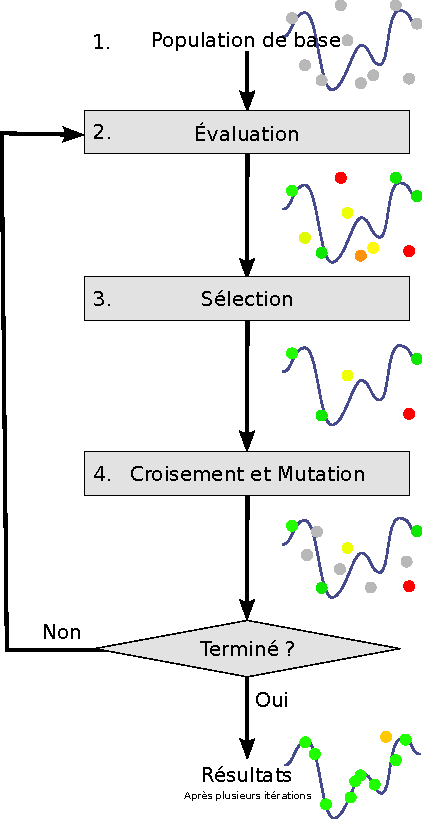
\includegraphics[width=.4\textwidth]{img/algo_genetique.pdf}
  \caption{Schéma des étapes d'un algorithme génétique}
  \label{cache:fig:genetic_schema}
\end{figure}

La Figure~\ref{cache:fig:genetic_schema} illustre le mécanisme de fonctionnement d'un algorithme génétique.

Un algorithme génétique démarre en utilisant une population d'individus de base qui est représentée dans l'étape 1 sur la Figure~\ref{cache:fig:genetic_schema}.
Dans le cas du \ac{RPCA}, la population initiale est générée en tirant un $c_u$ au hasard entre $\cmin$ et $\cmax$ afin d'éviter les solutions inadmissibles d'emblée.

Cette population va subir un traitement systématique pendant un nombre fini d'itérations appelées \emph{générations}.
Ce traitement est composé de plusieurs étapes: évaluation des aptitudes de chaque solution, sélection des meilleurs individus, croisement et application des mutations.
Ces étapes permettent de créer une nouvelle population et ce cycle recommence pendant un nombre fixé de générations ou bien lorsque les populations sont acceptables.
Les meilleures solutions qui ont été sélectionnées au fil des générations sont données comme solution au problème et constituent une approximation du front de Pareto.

\subsection{Aptitude}
\label{cache:fitness}

La fonction d'aptitude (ou ``fitness'' en anglais) évalue à quel point une solution est admissible ou non et si elle l'est quelle est son efficacité.
L'algorithme génétique n'impose aucune hypothèse sur cette fonction qui doit seulement renvoyer un réel.

Déterminer une fonction d'aptitude est la partie la plus liée au problème multi-objectifs lors de la conception d'un algorithme génétique; les autres étapes étant relativement génériques d'un problème à l'autre.

Pour chaque $\mathcal{C}$, il y a deux critères à prendre en compte: la durée de vie minimale du \ac{LLN} qu'il permet d'obtenir et la satisfaction que les utilisateurs auront si ce $\mathcal{C}$ est utilisé.
Soit $\mathcal{L}(\mathcal{C})$ la durée de vie obtenue dans le pire cas c'est-à-dire quand $r_u = c_u$.
Soit $\Gamma(\mathcal{C})$ qui est la satisfaction moyenne ressentie par l'utilisation et qui est définie comme: $\Gamma(\mathcal{C}) = \frac{1}{N}\sum_{u} \gamma_u$.

Soit $f$ la fonction d'aptitude obtenue en normalisant les grandeurs $\Gamma(\mathcal{C})$ et $\mathcal{L(C)}$ entre $0$ et $1$:

\begin{align}
  f(\mathcal{C}) &= \frac{1}{2} \left(
    \frac{\Gamma(\mathcal{C}) - \Gamma(\mathcal{C}_{\textrm{min}})}
    {\Gamma(\mathcal{C}_{\textrm{max}}) - \Gamma(\mathcal{C}_{\textrm{min}})}
    +
    \frac{\mathcal{L(C)} - \mathcal{L(C_{\textrm{min}})}}
    {\mathcal{L(C_{\textrm{max}})} - \mathcal{L(C_{\textrm{min}})}}\right)
    \label{cache:eq:fitness1}\\
                 &= \frac{1}{2} \left(\Gamma(\mathcal{C})
      +\frac{\mathcal{L(C)} - \mathcal{L(C_{\textrm{min}})}}
      {\mathcal{L(C_{\textrm{max}})} - \mathcal{L(C_{\textrm{min}})}}\right)
  \label{cache:eq:fitness2}
\end{align}

Or, puisque $\Gamma(\mathcal{C}_{\textrm{min}}) = 0$ et $\Gamma(\mathcal{C}_{\textrm{max}}) = 1$,  l'équation~\eqref{cache:eq:fitness1} peut être simplifiée pour obtenir~\eqref{cache:eq:fitness2}.
D'autre part, la moyenne permet de ne pas privilégier des solutions conservatrices en énergie au détriment d'autres.

\subsection{Sélection}
\label{cache:selection}

Le processus de sélection utilise l'aptitude précédemment définie pour sélectionner les solutions qui vont se ``reproduire''.
Un des écueils courant des méthodes d'optimisation multi-objectifs génétique est de rester bloqué dans un sous-ensemble de solutions très homogènes.
Dans le cas du \ac{RPCA} cela voudrait dire que les solutions resteraient fixées sur un point localement optimal, or l'objectif est d'avoir une population aussi diversifiée que possible afin de pouvoir changer rapidement de solution en cas de changement de trafic.

Ainsi, à niveau d'aptitudes semblables, les solutions les plus éloignées les unes des autres devraient être sélectionnées.
C'est la méthode utilisée par NSGA-II~\cite{deb1999niched} qui est élitiste: les meilleures solutions sont retenues d'une génération à l'autre et forment les élites.
Cependant, cette sélection s'accompagne d'une préservation de la diversité qui privilégie les solutions éloignées les unes des autres.

Pour fonctionner, NSGA-II utilise une métrique d'estimation de densité qui va estimer la distance moyenne qui le sépare des autres solutions.
Puis lorsque deux solutions doivent être départagées lors d'une sélection, celle qui est la plus éloignée des autres solutions sera choisie.
Cette méthode de sélection permet d'avoir un large ensemble de solutions et sera celle utilisée pour le reste du chapitre.

D'autre part, cette méthode garde en mémoire les meilleures solutions vues à chaque génération (``hall of fame'' en anglais) afin de ne perdre aucune solution intéressante même si par le hasard des sélections elle n'est pas sélectionnée.

\subsection{Croisement \& Mutation}
\label{cache:mutation}

Les algorithmes génétiques utilisent des opérateurs afin d'altérer les populations de solutions existantes pour en former de nouvelles et explorer ainsi l'espace des solutions.
Il existe essentiellement deux opérateurs génétiques: le croisement et la mutation.

Comme de nombreuses méta-heuristiques, ces mécanismes très hétérogènes peuvent être complexes à configurer, car de nombreux paramètres sont disponibles.
Cependant, l'utilisation d'algorithmes de sélection élitiste permet de mitiger cette complexité, car les meilleures solutions sont gardées en mémoire dans le ``hall of fame''.
Ainsi, les mécanismes de mutation et de croisement peuvent être configurés pour être  ``exploratoires'', tandis que les mécanismes de sélection s'occupent de garder les meilleures solutions.

\subsubsection{Mutation}

La mutation est un processus de transformation qui est appliquée sur chaque individu avec une probabilité $p_m$ à chaque génération.
Ce processus modifie les gènes d'une solution (en l’occurrence les $c_u$) dans les bornes inférieures et supérieures admissibles (en l’occurrence $\cmin$ et $\cmax$).

Le reste de cette thèse utilise la méthode préconisée par les auteurs de NSGA-II qui est une mutation polynomiale qui utilise une distribution polynomiale définie entre $\cmin$ et $\cmax$~\cite{deb2014analysing}.

\subsubsection{Croisement}

Le croisement est un mécanisme d'exploration qui prend deux sous-ensembles de $c_u$, $c'_u$ appartenant à deux solutions distinctes $\mathcal{C}$ et $\mathcal{C}'$ et les échangent à la génération suivante.

\begin{figure}[ht]
  \centering
  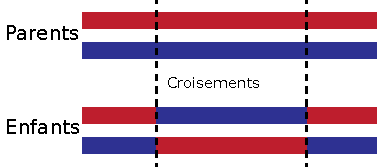
\includegraphics[scale=1]{img/crossover.pdf}
  \caption{Croisement de deux individus par points doubles}
  \label{cache:fig:crossover}
\end{figure}

La Figure~\ref{cache:fig:crossover} illustre ce mécanisme de croisement à point double qui sélectionne deux points et échange l'ensemble des gènes entre ces deux points.
C'est le mécanisme de croisement qui est recommandé pour être appliqué à NSGA-II ~\cite{Luke2013Metaheuristics} et qui sera utilisé dans cette thèse.

\section{Validation expérimentale}
\label{cache:validation}

Le \ac{RPCA} est évalué dans le scénario suivant: 12 serveurs \ac{CoAP} utilisant la bibliothèque Erbium~\cite{kovatsch2011low} sont déployés.
Ces nœuds utilisent Contiki~\cite{dunkels2004contiki} comme système d'exploitation et sont émulés via Cooja~\cite{cooja}.
Cooja les émule comme des TmoteSky fonctionnant avec un processeur de type MSP430 et utilisant pour communiquer une puce radio CC2420 dont les consommations énergétiques sont connues~\cite{Polastre05}.

\begin{figure}[ht]
  \centering
  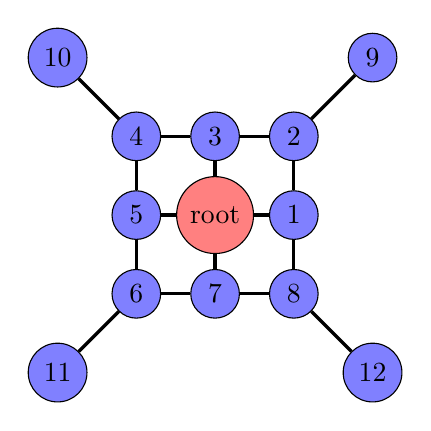
\begin{tikzpicture}
  % définition des styles
  \tikzstyle{root}=[circle, draw, fill=red!50,text=black]
  \tikzstyle{node}=[circle, draw, fill=blue!50,text=black]

  \tikzstyle{estun}=[-,>=latex,very thick]
  % les nœuds
  \node[root] (root) at (0, 0) {root};

  \node[node] (1) at (1,0) {1};
  \node[node] (2) at (1,1) {2};
  \node[node] (3) at (0,1) {3};
  \node[node] (4) at (-1, 1) {4};
  \node[node] (5) at (-1, 0) {5};
  \node[node] (6) at (-1, -1) {6};
  \node[node] (7) at (0, -1) {7};
  \node[node] (8) at (1, -1) {8};

  \node[node] (9) at (2, 2) {9};
  \node[node] (10) at (-2, 2) {10};
  \node[node] (11) at (-2, -2) {11};
  \node[node] (12) at (2, -2) {12};

  \draw[estun] (root)--(1);
  \draw[estun] (root)--(3);
  \draw[estun] (root)--(5);
  \draw[estun] (root)--(7);

  \draw[estun] (1)--(2);
  \draw[estun] (2)--(3);
  \draw[estun] (3)--(4);
  \draw[estun] (4)--(5);
  \draw[estun] (5)--(6);
  \draw[estun] (6)--(7);
  \draw[estun] (7)--(8);
  \draw[estun] (8)--(1);

  \draw[estun] (2)--(9);
  \draw[estun] (4)--(10);
  \draw[estun] (6)--(11);
  \draw[estun] (8)--(12);

  \end{tikzpicture}

  \caption{Topologie radio considérée pour la validation expérimentale du \ac{RPCA}.}

  \label{cache:fig:topology}
\end{figure}

La Figure~\ref{cache:fig:topology} représente la topologie radio utilisée où un lien signifie que les nœuds peuvent être en communication radio l'un avec l'autre.
Les nœuds utilisent le protocole \ac{RPL}~\cite{rfc6550} pour établir une topologie de routage qui est connue par le routeur de bordure afin de modéliser la durée de vie du réseau.

\begin{table*}[ht]
\centering
\begin{tabular}{|l|c|c|}
\hline
Débit de transmission & $R$ & 250 kbps \\
\hline
Intervalle entre deux tentatives de préambules & $T_\pkt$ & 0.4 ms \\
\hline
Temps d'une période MAC & $T_\cycle$ & 0.244 s\\
\hline
Temps d'une période active & $T_\act$ & 40 ms\\
\hline
Temps pour détecter un paquet \ac{ACK} & $T_\detect$ & 0.16 ms \\
\hline
Taille d'une requête CoAP (\texttt{GET}) & $L_\req$ & 87 octets\\
\hline
Taille d'une réponse CoAP & $L_\ans$ & 96 octets \\
\hline
Temps pour transmettre un \ieee{} \ac{ACK} & $T_\ack$ & 0.608 ms  \\
\hline
Puissance consommée lors de la transmission & $P_\tx $ & 0.0511 W  \\
\hline
Puissance consommée lors de la réception & $P_\rx $ & 0.0588 W  \\
\hline
Puissance consommée lors du sommeil & $P_\sleep$ & $2.4\cdot 10^{-7}$ W \\
\hline
Nombre de nœuds dans le \ac{LLN}  & $N$ & 12 \\
\hline
Nombre de run par configuration &  & 10  \\
\hline
Nombre de requêtes \ac{CoAP} traité par nœuds &  & 50 \\
\hline
\end{tabular}
\caption{Paramètres utilisés dans les simulations.}

\label{cache:table:sim_parameters}
\end{table*}

Le tableau~\ref{cache:table:sim_parameters} donne les paramètres numériques utilisés lors de l'expérience.
Les nœuds utilisent ContikiMAC comme mécanisme de cycle de veille afin d'économiser de l'énergie et démarrent tous avec la même énergie initiale.
La consommation énergétique du réseau est obtenue en utilisant la topologie et la modélisation de ContikiMAC précédemment introduite.
La durée de vie du \ac{LLN} est calculée comme l'intervalle de temps entre son démarrage et la perte de son premier nœud.

Le \ac{RPCA} met en cache les réponses rendues par les nœuds afin de les mettre à disposition pour une éventuelle autre demande entrante.
Une fois la topologie et le trafic connus, la résolution du problème multi-objectifs est lancée et les différents $\mathcal{C}$ sont calculés.
Le \ac{RPCA} a suffisamment de mémoire pour retenir toutes les réponses pour chaque \ac{URI} disponible dans le réseau.
La passerelle est toujours allumée, car non contrainte en énergie et assure une connexion permanente à un réseau local conventionnel.

Des requêtes \ac{HTTP} sont envoyées vers le \ac{RPCA} puis sont traduites vers une requête \ac{CoAP} et inversement en utilisant la bibliothèque Californium~\cite{kovatsch2014californium}.
Le trafic ne démarre que lorsque la topologie de routage est établie.

Le temps entre chaque requête est modélisé par un temps d'attente exponentiel de paramètre $\lambda_u$ et $\forall u, \lambda_u = \lambda$.
Ainsi le temps entre chaque requête correspond à $r_u$ pour le nœud qui héberge la ressource $u$.
Afin d'avoir une empreinte mémoire faible, chaque serveur n'a qu'une seule ressource et afin de faciliter l'analyse sera un texte de taille fixe ne causant pas de fragmentations.
Il est supposé que le trafic est suffisamment faible pour que les pertes de paquets soient négligeables.

\subsection{Compromis entre durée de vie et satisfaction utilisateur}

Le \ac{RPCA} est configuré pour utiliser un algorithme génétique pour trouver les solutions avec les paramètres suivants:

\begin{table*}[ht]
\centering
\begin{tabular}{|l|c|c|}
\hline
Population & $P$ & 100 \\
\hline
Probabilité d'accouplement & $p_c$ & 0.5 \\
\hline
Probabilité de mutation & $p_m$ & 0.2 \\
\hline
Nombre de générations & $n_g$ & 50 \\
% \hline
% Index de la distribution de mutation & $\eta_m$ & 20 \\
\hline
Temps de validité en cache minimal & $\cmin$ & 1s \\
\hline
Temps de validité en cache maximal & $\cmax$ & 9s \\
% \hline
% Taux de requêtes entrantes & $\lambda$ & 1 \\
\hline
\end{tabular}
\caption{Paramètres utilisés dans l'optimisation multi-objectifs.}

\label{cache:table:nsga2_parameters}
\end{table*}

\begin{figure}[ht]
  \centering

 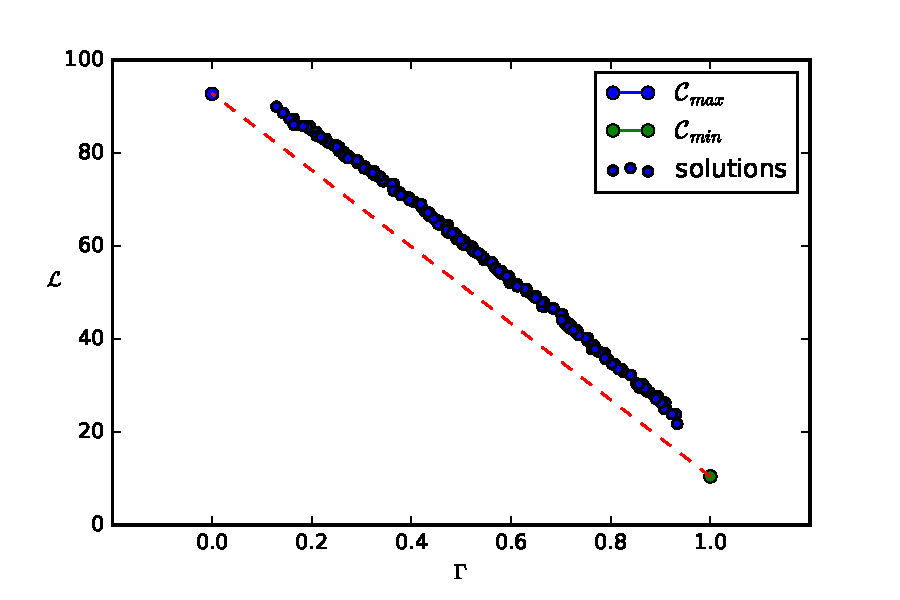
\includegraphics[width=.7\textwidth]{img/pareto.pdf}

 \caption{Front de Pareto pour le scénario envisagé.}

 \label{cache:fig:paretofront}

\end{figure}

Les probabilités d'accouplement et de mutation sont laissées aux valeurs recommandées par les créateurs de NSGA-II.
Le nombre de générations et la taille de population sont choisis afin d'avoir un temps de calcul modeste et d'obtenir une approximation du front de Pareto rapide.
La Figure~\ref{cache:fig:paretofront} montre la population de solutions produites par l'algorithme génétique.
Chaque point solution est un $\mathcal{C}$ contenant l'ensemble des $c_u$.
Ces points forment une approximation du front de Pareto qui représente les solutions optimales et les durées de vie mesurées en jours.

Les poins $\mathcal{C}_{min}$ et $\mathcal{C}_{max}$ sont également présentés afin de montrer les bornes possibles des solutions.
Ainsi  $\mathcal{C}_{min}$ garanti une fraîcheur aussi élevée que possible, mais raccourcit la durée de vie alors que $\mathcal{C}_{max}$ garanti une durée de vie aussi longue que possible.

Une valeur haute de $c_u$ sera utilisée pour des nœuds ayant peu d'énergie.
Par contre, une valeur $c_u$ petite sera pour des informations devant être aussi récentes que possible.

\subsection{Cache hit}

\begin{figure}[ht]
  \centering
  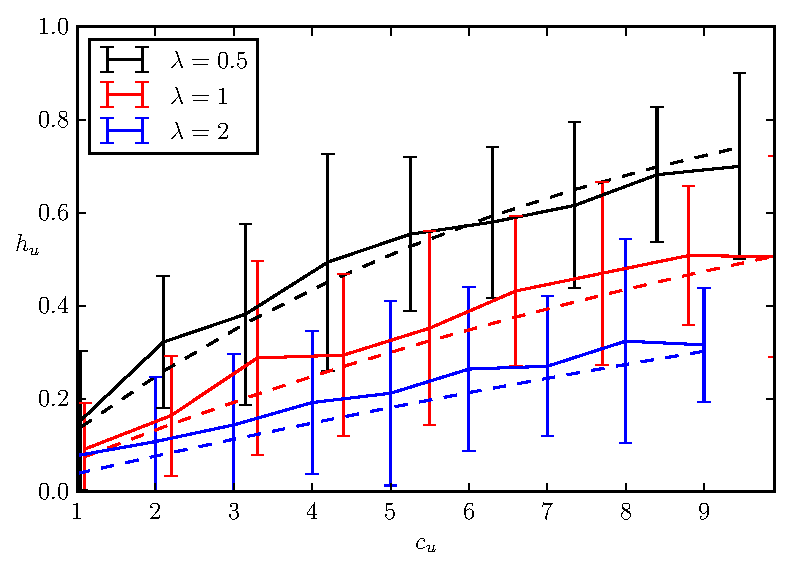
\includegraphics[width=.5\textwidth]{img/new_cachinghit.pdf}
  \caption{Évolution du cache hit en fonction de la durée de vie}
  \label{cache:fig:hit}
\end{figure}

La Figure~\ref{cache:fig:hit} illustre l'évolution du nombre de requêtes servies par le cache (hit) en fonction de la durée de vie des requêtes $c_u$ choisies.
La simulation (traits pleins) est comparée à la modélisation théorique (lignes en pointillés cf~\eqref{cache:eq:cache_hit}) pour différentes valeurs de paramètres $\lambda$ sur la Figure~\ref{cache:fig:hit}.
Afin de simplifier la représentation visuelle, le graphique montre quels sont les résultats obtenus lorsque tous les $c_u$ et $\lambda_u$ sont égaux entre eux.

Plus $c_u$ est grand par rapport à $T_u = \frac{1}{\lambda_u}$, plus le cache est efficace, car la probabilité que la requête soit servie par le \ac{RPCA} augmente épargnant ainsi aux nœuds du \ac{LLN} de les traiter.

Quand $c_u$ est petit devant $T_u = \frac{1}{\lambda_u}$, la fréquence de requête est plus faible que le temps de vie dans le cache.
Le cache est ici inefficace, car une réponse n'y vit pas assez longtemps pour être susceptible d'être utilisée.

Ainsi l'efficacité d'un cache n'est pas seulement liée au temps de vie d'une requête, mais également à son adéquation avec le trafic qu'il reçoit.

\subsection{Amélioration de la durée de vie}

\begin{figure}[ht]
  \centering
  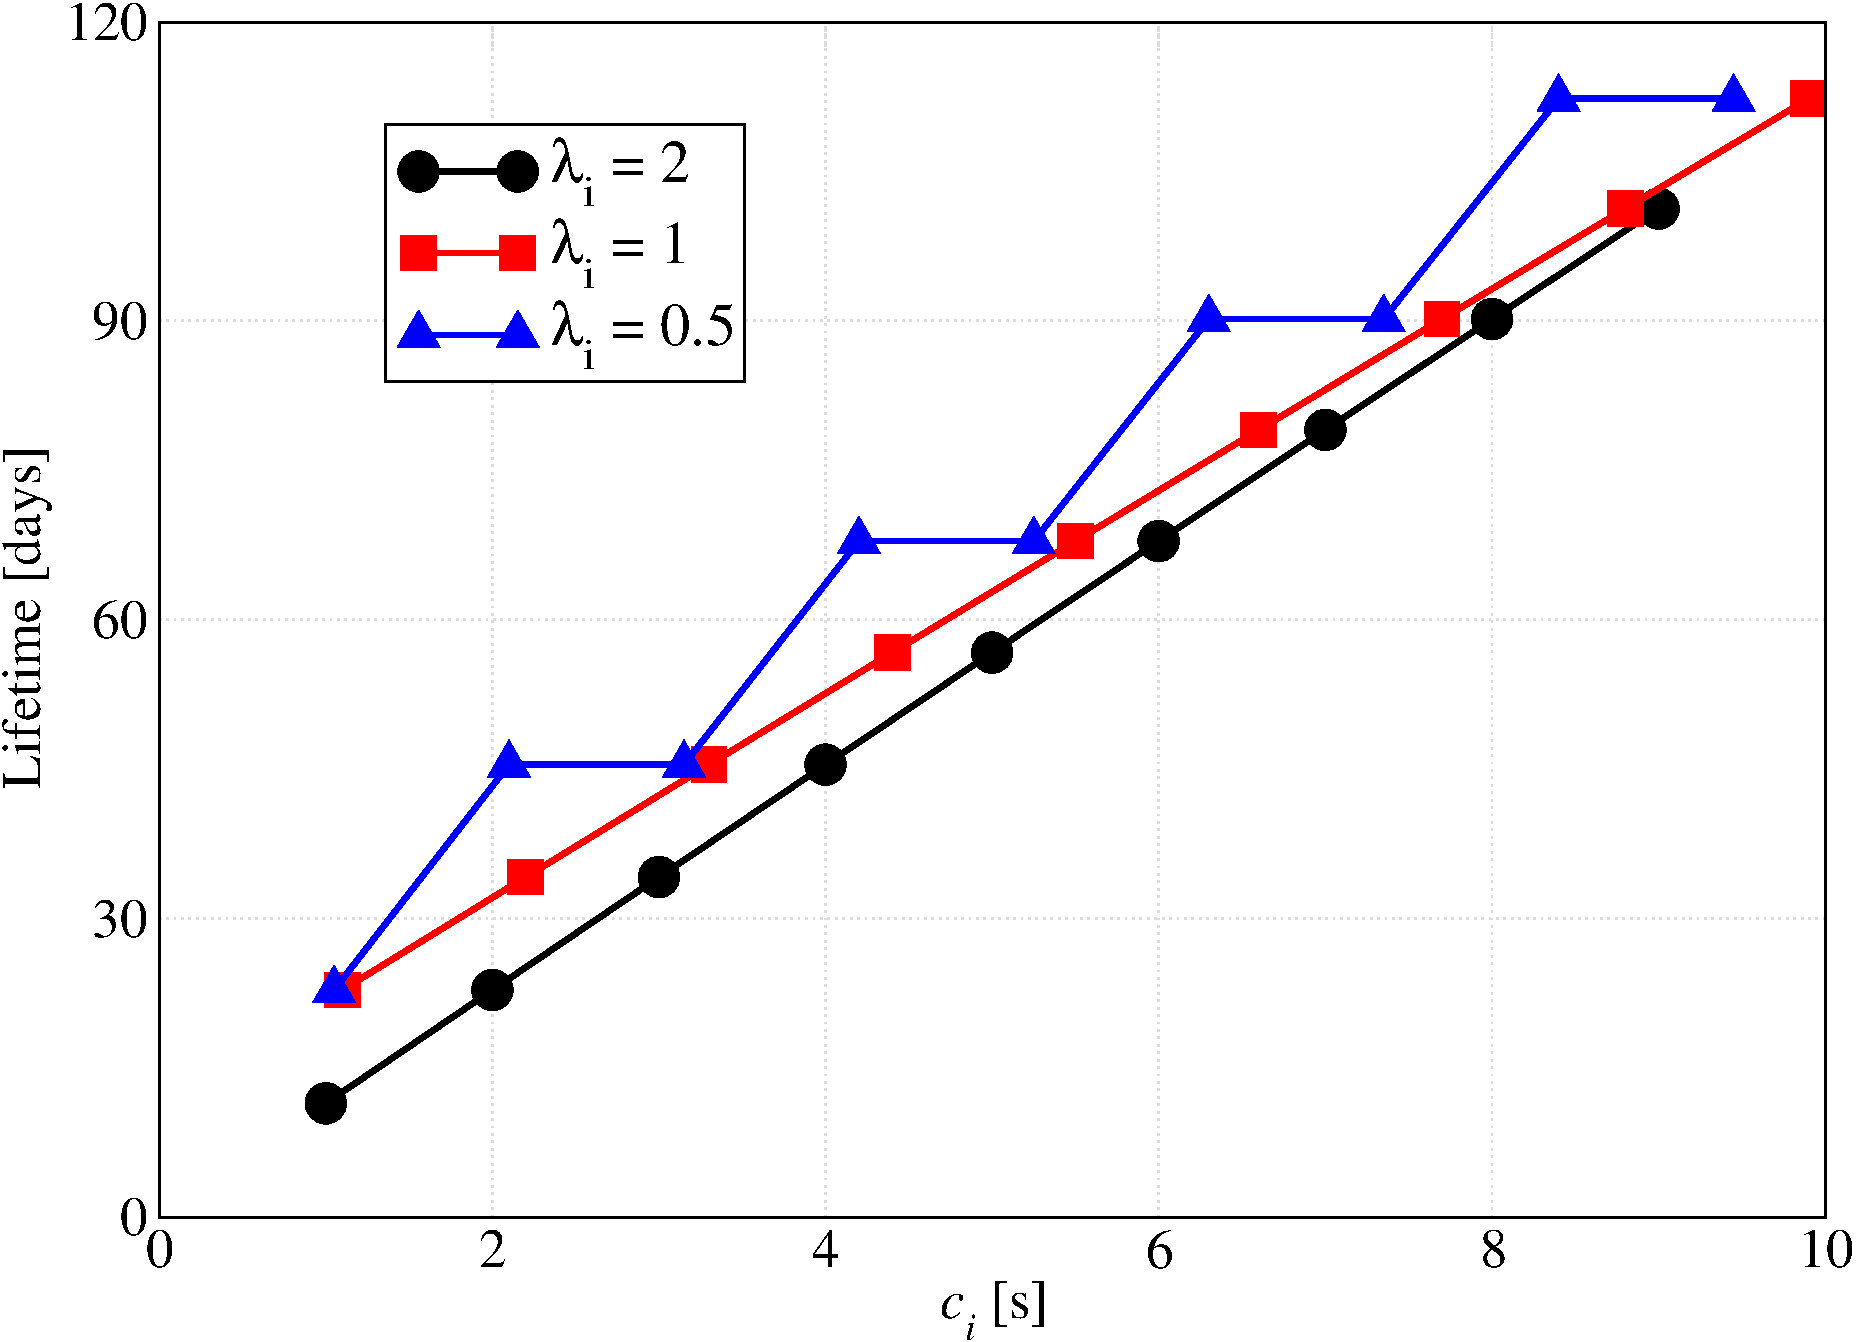
\includegraphics[width=0.455\textwidth]{img/lifetime.pdf}
  \caption{Évolution de la durée de vie théorique en fonction des $c_u$}
  \label{cache:fig:lifetime}
\end{figure}

La Figure~\ref{cache:fig:lifetime} illustre la durée de vie théorique obtenue pour le \ac{LLN} pour différentes configurations de cache identiques.
Il est observé que plus les temps de cache sont élevés, plus la durée de vie du \ac{LLN} est élevée ce qui est attendu, car une grande durée de vie implique que moins de requêtes applicatives sont gérées par le \ac{LLN}.

\section{Conclusion}
\label{cache:conclusion}

% Résumé

Ce chapitre montre comment un \ac{RPCA} permet d'optimiser l'utilisation des ressources d'un \ac{LLN} en adaptant la quantité de requêtes applicatives admises dans le \ac{LLN}.
Ce mécanisme utilise une modélisation de la consommation énergétique et de la satisfaction des utilisateurs afin de fournir un temps de vie pour toutes les réponses
aux requêtes que le \ac{RPCA} doit gérer.

% Avantages

Un \ac{RPCA} change dynamiquement la quantité de requêtes applicatives entrantes dans un \ac{LLN} afin d'économiser ses ressources d'une part et d'accélérer le traitement des requêtes d'autre part.
De plus, le \ac{RPCA} utilise une estimation de la durée de vie pour aider l'administrateur d'un \ac{LLN} à trouver une configuration adaptée pour les objectifs de durée de vie visés.

% Limitations

L'utilisation d'algorithme génétique permet d'avoir un mécanisme général pouvant être appliqué à n'importe quelle situation.
Cependant, cette méthode n'offre pas de garanties de convergence vers le front de Pareto pour un nombre de générations donné.
Des méthodes plus spécifiques utilisant notamment une hypothèse de convexité sur les fonctions objectifs permettrait d'aller plus vite.

% Amélioration

Une piste d'amélioration possible consisterait à tester d'autres méthodes de résolutions d'optimisations multi-objectifs afin de comparer avec d'autres mécanismes présentant la même flexibilité.
Cependant, la tâche est complexe, car le nombre d'heuristiques disponibles dans la littérature est très élevé et implémenter ces heuristiques est long et met en jeu de nombreux paramètres de configuration rendant cette exploration difficile.

Une autre amélioration peut également être envisagée pour fournir un modèle de satisfaction des utilisateurs prenant en compte le nombre de requêtes reçues.
Ainsi, le \ac{RPCA} pourrait utiliser une modélisation de la satisfaction des utilisateurs tenant compte des popularités respectives des différentes \ac{URI}.

Enfin, un \ac{RPCA} pourrait également être étendu afin de gérer la fréquence d'envois des observations en provenance des nœuds.
Dans certains \ac{LLN}s, les nœuds envoient périodiquement des notifications à la passerelle afin qu'elle puisse redistribuer cette notification aux abonnés intéressés.
N'avoir que la passerelle comme abonné allège la charge qu'un nœud doit gérer.
Le \ac{RPCA} pourrait configurer les nœuds pour réguler la fréquence d'envoi des notifications.
L'objectif serait de trouver le bon compromis entre la satisfaction des utilisateurs qui veulent des informations régulièrement et les nœuds qui veulent envoyer aussi peu de notifications que possible.

\section*{Publications}

\begin{itemize}
  \item Rémy Leone, Paolo Medagliani et Jérémie Leguay.
    \newblock {Optimizing QoS in Wireless Sensors Networks using a Caching Platform}.
    \newblock {\em {Sensornets 2013}}, page~56, Barcelone, Espagne, Février 2013.

  \item Rémy Leone, Paolo Medagliani et Jérémie Leguay.
    \newblock {Optimisation de la qualité de service par l'utilisation de mémoire cache}
    \newblock 15{\`e}mes Rencontres Francophones sur les Aspects Algorithmiques des T{\'e}l{\'e}communications

\end{itemize}